\documentclass[]{article}
\usepackage[T1]{fontenc}
\usepackage{lmodern}
\usepackage{amssymb,amsmath}
\usepackage{ifxetex,ifluatex}
\usepackage{fixltx2e} % provides \textsubscript
% use upquote if available, for straight quotes in verbatim environments
\IfFileExists{upquote.sty}{\usepackage{upquote}}{}
\ifnum 0\ifxetex 1\fi\ifluatex 1\fi=0 % if pdftex
  \usepackage[utf8]{inputenc}
\else % if luatex or xelatex
  \ifxetex
    \usepackage{mathspec}
    \usepackage{xltxtra,xunicode}
  \else
    \usepackage{fontspec}
  \fi
  \defaultfontfeatures{Mapping=tex-text,Scale=MatchLowercase}
  \newcommand{\euro}{€}
\fi
% use microtype if available
\IfFileExists{microtype.sty}{\usepackage{microtype}}{}
\usepackage[margin=1in]{geometry}
\usepackage{color}
\usepackage{fancyvrb}
\newcommand{\VerbBar}{|}
\newcommand{\VERB}{\Verb[commandchars=\\\{\}]}
\DefineVerbatimEnvironment{Highlighting}{Verbatim}{commandchars=\\\{\}}
% Add ',fontsize=\small' for more characters per line
\usepackage{framed}
\definecolor{shadecolor}{RGB}{248,248,248}
\newenvironment{Shaded}{\begin{snugshade}}{\end{snugshade}}
\newcommand{\KeywordTok}[1]{\textcolor[rgb]{0.13,0.29,0.53}{\textbf{{#1}}}}
\newcommand{\DataTypeTok}[1]{\textcolor[rgb]{0.13,0.29,0.53}{{#1}}}
\newcommand{\DecValTok}[1]{\textcolor[rgb]{0.00,0.00,0.81}{{#1}}}
\newcommand{\BaseNTok}[1]{\textcolor[rgb]{0.00,0.00,0.81}{{#1}}}
\newcommand{\FloatTok}[1]{\textcolor[rgb]{0.00,0.00,0.81}{{#1}}}
\newcommand{\CharTok}[1]{\textcolor[rgb]{0.31,0.60,0.02}{{#1}}}
\newcommand{\StringTok}[1]{\textcolor[rgb]{0.31,0.60,0.02}{{#1}}}
\newcommand{\CommentTok}[1]{\textcolor[rgb]{0.56,0.35,0.01}{\textit{{#1}}}}
\newcommand{\OtherTok}[1]{\textcolor[rgb]{0.56,0.35,0.01}{{#1}}}
\newcommand{\AlertTok}[1]{\textcolor[rgb]{0.94,0.16,0.16}{{#1}}}
\newcommand{\FunctionTok}[1]{\textcolor[rgb]{0.00,0.00,0.00}{{#1}}}
\newcommand{\RegionMarkerTok}[1]{{#1}}
\newcommand{\ErrorTok}[1]{\textbf{{#1}}}
\newcommand{\NormalTok}[1]{{#1}}
\usepackage{graphicx}
% Redefine \includegraphics so that, unless explicit options are
% given, the image width will not exceed the width of the page.
% Images get their normal width if they fit onto the page, but
% are scaled down if they would overflow the margins.
\makeatletter
\def\ScaleIfNeeded{%
  \ifdim\Gin@nat@width>\linewidth
    \linewidth
  \else
    \Gin@nat@width
  \fi
}
\makeatother
\let\Oldincludegraphics\includegraphics
{%
 \catcode`\@=11\relax%
 \gdef\includegraphics{\@ifnextchar[{\Oldincludegraphics}{\Oldincludegraphics[width=\ScaleIfNeeded]}}%
}%
\ifxetex
  \usepackage[setpagesize=false, % page size defined by xetex
              unicode=false, % unicode breaks when used with xetex
              xetex]{hyperref}
\else
  \usepackage[unicode=true]{hyperref}
\fi
\hypersetup{breaklinks=true,
            bookmarks=true,
            pdfauthor={},
            pdftitle={Regression Models Course Project Report},
            colorlinks=true,
            citecolor=blue,
            urlcolor=blue,
            linkcolor=magenta,
            pdfborder={0 0 0}}
\urlstyle{same}  % don't use monospace font for urls
\setlength{\parindent}{0pt}
\setlength{\parskip}{6pt plus 2pt minus 1pt}
\setlength{\emergencystretch}{3em}  % prevent overfull lines
\setcounter{secnumdepth}{0}

\title{Regression Models Course Project Report}
\author{}
\date{}

\begin{document}

\begin{center}
\huge Regression Models Course Project Report \\[0.2cm]
\end{center}
\normalsize


\subsection{Martin Hediger}\label{martin-hediger}

\subsubsection{Executive Summary}\label{executive-summary}

This short report analyses if 1) automatic or manual transmission
results in larger miles-per-gallon (mpg) and 2) quantifies the effect of
manual or automatic transmission on mpg in the cars from the
\texttt{mtcars} dataset.\\Automatic transmission vehicles appear to be
less efficient than manual transmission vehicles (Fig. ``box-scat'' A).
A linear relationship between miles-per-gallon range and car weight for
both automatic and manual transmission vehicles is found (Fig.
``box-scat'' B). Inference of a linear model of the form
$mpg_i = \beta_0 + \gamma \cdot (am_i \cdot wt) + \beta_1 \cdot wt_i + e_i$
for the dummy variable $am_i$ (0: auto, 1: man) indicates that the
dependence of $mpg$ on $wt$ is not different for the cars with automatic
and manual transmission.

\subsubsection{Exploratory Analysis}\label{exploratory-analysis}

As an initial test, dependence of \texttt{mpg} on \texttt{wt} is
analysed.\\\href{https://github.com/mzhKU/regmods_course_project/blob/master/box-scat.R}{\texttt{box-scat}}
A: Boxplot, B: Scatterplot of \texttt{mpg} against \texttt{wt}.

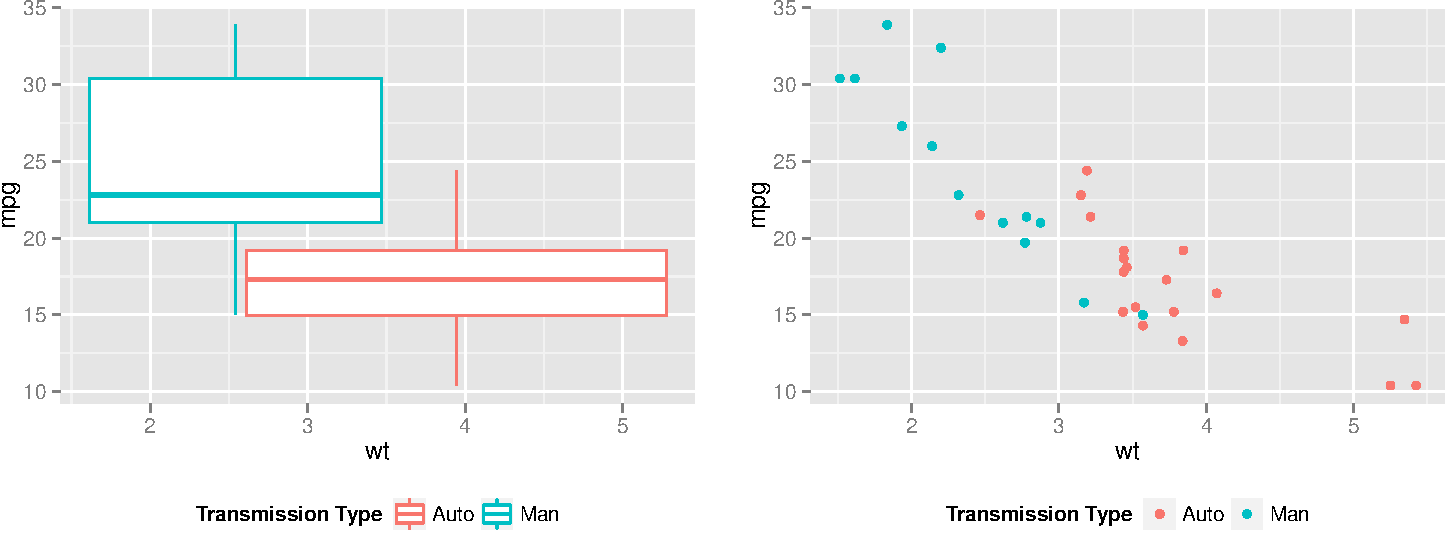
\includegraphics{./article_files/figure-latex/unnamed-chunk-1.pdf}

\href{https://github.com/mzhKU/regmods_course_project/blob/master/multiplot.R}{Source
code for the panel plot}.

According to the boxplot, automatic cars have lower MPG (and possibly
lower variance in the data). Importantly, the relationships appear
linear and no outliers which could affect correlation values are
identified. The only aspect which is slightly problematic is the limited
dataset size (n=32).\\It is noted that apparently most cars with
automatic transmission also are heavier which possibly confounds the
observation, this would be subject to further research.

\subsubsection{Results}\label{results}

\textbf{Question 1: Which transmission type has higher MPG?}\\Based on
the exploratory analysis above, it is found that on average the
difference between MPG(auto) and MPG(man) is around 7.2449
miles-per-gallon
(=\texttt{mean(mtcars{[}mtcars\$am==1, "mpg"{]}) - mean(mtcars{[}mtcars\$am==0, "mpg"{]})}).

\textbf{Question 2: Quantification of MPG-difference between
transmission types}\\MODEL 1\\In the full model
\texttt{lm(mpg \textasciitilde{} . + factor(am), data=mtcars)} there is
no strong evidence against the null hypothesis for any variable,
i.e.~that $H_{0, i} \neq 0$ where
$i \in \{cyl, disp, hp, drat, wt, qsec, vs, am, gear, carb\}$, that is
all p-values are larger than any accepted significance level.

Theory suggests that the smallest reasonable model should be employed,
so based on the collectively large p-values for the different variables
in the full model, the variables \texttt{wt}, \texttt{am}, \texttt{qsec}
and \texttt{hp} are considered for a reduced model because of all
variables, these have lowest p-values.

MODEL 2\\It is tested if miles-per-gallon are sufficiently explained by
\texttt{wt}, \texttt{am}, \texttt{qsec} and \texttt{hp}.

A residual against fitted values plot (appendix) shows uniform
distribution and a Cook's distance plot confirms that no data point has
substantially stronger influence on the fit than the other points.

MODEL 3\\It is found that the evidence against \texttt{hp} being
different from zero is very weak (p-value 0.223). Therefore, in the last
model only \texttt{wt}, \texttt{am} and \texttt{qsec} remain.

There is strong evidence that the coefficient of \texttt{wt} is
different from zero (p-value \textless{}\textless{} 0.001).

Therefore, we perform inference using a Dummy variable in the model
$mpg = \hat{\beta_0} + \hat{\beta_1} \cdot wt + \hat{\gamma} \cdot (am_i \cdot wt)$
under the assumption that both (auto and manual cars) have the same
zero-weight MPG.

\begin{Shaded}
\begin{Highlighting}[]
\NormalTok{fit_4 <-}\StringTok{ }\KeywordTok{summary}\NormalTok{(}\KeywordTok{lm}\NormalTok{(mpg ~}\StringTok{ }\NormalTok{wt +}\StringTok{ }\KeywordTok{I}\NormalTok{(am*wt), }\DataTypeTok{data=}\NormalTok{mtcars))}
\NormalTok{fit_4$coefficients}
\end{Highlighting}
\end{Shaded}

\begin{verbatim}
##             Estimate Std. Error t value  Pr(>|t|)
## (Intercept)  38.8798     2.5094 15.4937 1.453e-15
## wt           -5.6895     0.6654 -8.5506 2.029e-09
## I(am * wt)   -0.4947     0.5156 -0.9595 3.452e-01
\end{verbatim}

The coefficients are interpreted as follows. The \texttt{wt} dependence
of automatic cars (\texttt{am} = 0) is such that for every unit in
\texttt{wt}, the MPG decreases by 5.7 units. However, given that the
p-value for the dummy variable \texttt{I(am*wt)} is around 0.34, it is
not plausible to believe that the \texttt{wt} dependence of manual cars
is different from automatic cars. This is illustrated in a figure in the
appendix where a single linear model can explain the MPG dependence of
both manual and automatic cars.

\subsubsection{Conclusion}\label{conclusion}

MPG is higher for manual cars and the \texttt{wt} dependence of MPG is
not different between automatic and manual cars.

\subsubsection{Appendix}\label{appendix}

Appendix Fig. S1: Residual against fitted plot and Cook's distance plots
(Model
2).\\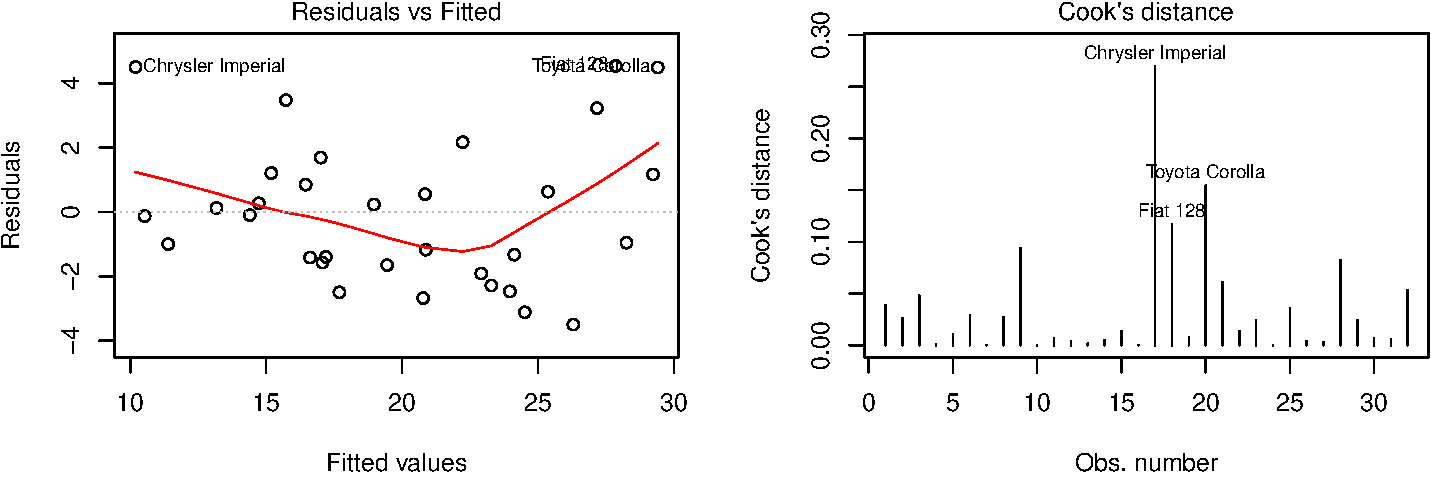
\includegraphics{./article_files/figure-latex/unnamed-chunk-6.pdf}

Appendix Fig. S2: Dummy Variable Analysis: Does MPG dependence on
\texttt{wt} differ for automatic and manual
cars?\\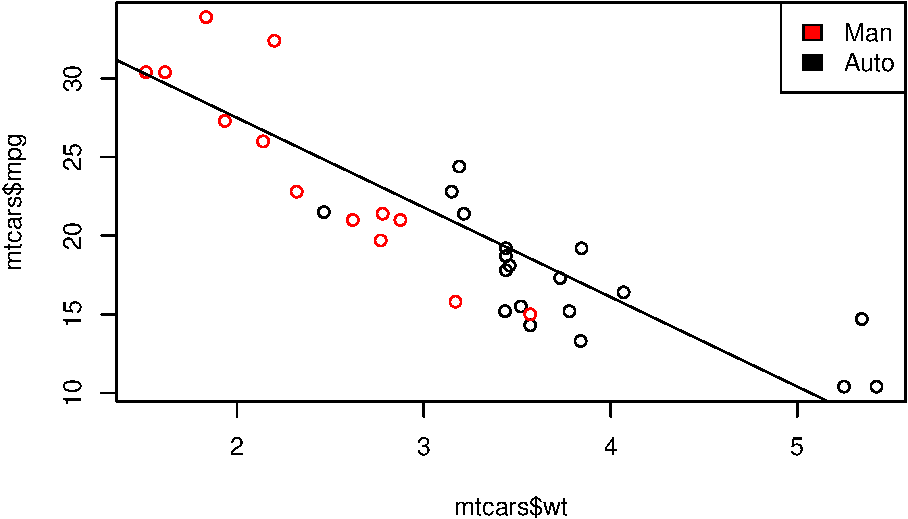
\includegraphics{./article_files/figure-latex/unnamed-chunk-7.pdf}

\end{document}
